% \documentclass[aspectratio=169,notes]{beamer}
\documentclass[aspectratio=169]{beamer}
\usetheme[faculty=phil]{fibeamer}
\usepackage{polyglossia}
\setmainlanguage{english} %% main locale instead of `english`, you
%% can typeset the presentation in either Czech or Slovak,
%% respectively.
\setotherlanguages{russian} %% The additional keys allow
%%
%%   \begin{otherlanguage}{czech}   ... \end{otherlanguage}
%%   \begin{otherlanguage}{slovak}  ... \end{otherlanguage}
%%
%% These macros specify information about the presentation
\title[IME]{Introduction to Mechanical Engineering, Lecture 8} %% that will be typeset on the
\subtitle{Design Thinking and Manufacturing  
\\ \   \\   
\ } %% title page.
\author{Oleg Bulichev}
%% These additional packages are used within the document:
\usepackage{ragged2e}  % `\justifying` text
\usepackage{booktabs}  % Tables
\usepackage{tabularx}
\usepackage{tikz}      % Diagrams
\usetikzlibrary{calc, shapes, backgrounds}
\usetikzlibrary{decorations.pathreplacing,calligraphy,calc,graphs}
\usepackage{amsmath, amssymb}
\usepackage{url}       % `\url`s
\usepackage{listings}  % Code listings
% \usepackage{subfigure}
\usepackage{floatrow}
\usepackage{subcaption}
\usepackage{mathtools}
\usepackage{todonotes}
\usepackage{fontspec}
\usepackage{multicol}
\usepackage{pdfpages}
\usepackage{wrapfig}
\usepackage{animate}
\usepackage{booktabs}
\usepackage{multirow}
% \usepackage{graphicx}
\usepackage{colortbl}

\graphicspath{{resources/}}
\frenchspacing

\setbeamertemplate{caption}[numbered]
\usetikzlibrary{graphs}

% \usepackage[backend=biber,style=ieee,autocite=footnote]{biblatex}
% \addbibresource{biblio.bib}
% \DefineBibliographyStrings{english}{%
%   bibliography = {References},}

\newcommand{\oleg}[2][] {\todo[color=red, #1] {OLEG:\\ #2}}
\newcommand{\fbckg}[1]{\usebackgroundtemplate{\includegraphics[width=\paperwidth]{#1}}}%frame background

\usepackage[framemethod=TikZ]{mdframed}
\newcommand{\dbox}[1]{
\begin{mdframed}[roundcorner=3pt, backgroundcolor=yellow, linewidth=0]
\vspace{1mm}
{#1}
\vspace{1mm}
\end{mdframed}
}

\begin{document}
\setlength{\abovedisplayskip}{0pt}
\setlength{\belowdisplayskip}{0pt}
\setlength{\abovedisplayshortskip}{0pt}
\setlength{\belowdisplayshortskip}{0pt}

\fbckg{fibeamer/figs/title_page.png}
\frame[c]{\setcounter{framenumber}{0}
    \usebeamerfont{title}%
    \usebeamercolor[fg]{title}%
    \begin{minipage}[b][6.5\baselineskip][b]{\textwidth}%
        \textcolor{black}{\raggedright\inserttitle}
    \end{minipage}
    % \vskip-1.5\baselineskip

    \usebeamerfont{subtitle}%
    \usebeamercolor[fg]{framesubtitle}%
    \begin{minipage}[b][3\baselineskip][b]{\textwidth}
        \raggedright%
        \insertsubtitle%
    \end{minipage}
    \vskip.25\baselineskip
}
%   \frame[c]{\maketitle}

\fbckg{fibeamer/figs/common.png}

\note{\scriptsize \begin{itemize}
        \item \
    \end{itemize}}

\begin{frame}[c]{}
    \framesubtitle{}
        \LARGE \centering
        What things do you consider when designing a part?
    \end{frame}

\begin{frame}[c]{Some properties to consider when designing a part}
\framesubtitle{}
\begin{table}[H]
    \LARGE
    \centering
    \begin{tabular}{|c|c|}
    \hline
        \textbf{Shape of the part} & \textbf{Temperature specs} \\ \hline
        Forces affecting the part & Post processing \\ 
        Shape & Mating and jointing \\ 
        Material & Scale of manufacturing \\ 
        Surface finish & Manufacturing cost \\ \hline
    \end{tabular}
\end{table}
\end{frame}

\begin{frame}[c]{}
    \framesubtitle{}
        \LARGE \centering
        What manufacturing methods do you know? 
    \end{frame}

    \begin{frame}[c]{Main types of manufacturing}
        \framesubtitle{Seif's classification}
        \begin{table}[H]
            \LARGE
            \centering
            \begin{tabular}{|c|c|}
            \hline
            Additive & Subtractive  \\ \hline
            Formative & Casting/Molding \\ \hline
            \end{tabular}
        \end{table}
        \end{frame}

\begin{frame}[t]{Main types of manufacturing}
\framesubtitle{}
    \vspace{-0.6cm}
    \begin{figure}[H]
        \centering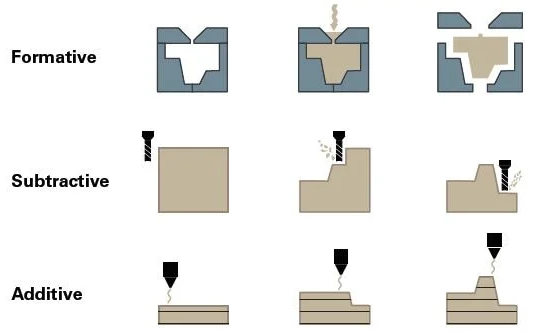
\includegraphics[height=6.5cm,width=1\textwidth,keepaspectratio]{fig1.png}
        \label{fig:fig1.png}
    \end{figure}
\end{frame}

\begin{frame}[c]{}
    \framesubtitle{}
        \LARGE \centering
        Now, what machines fall under these manufacturing types? 
    \end{frame}

\begin{frame}[t]{Manufactoring Processes types}
\framesubtitle{}
    \vspace{-0.6cm}
    \begin{figure}[H]
        \centering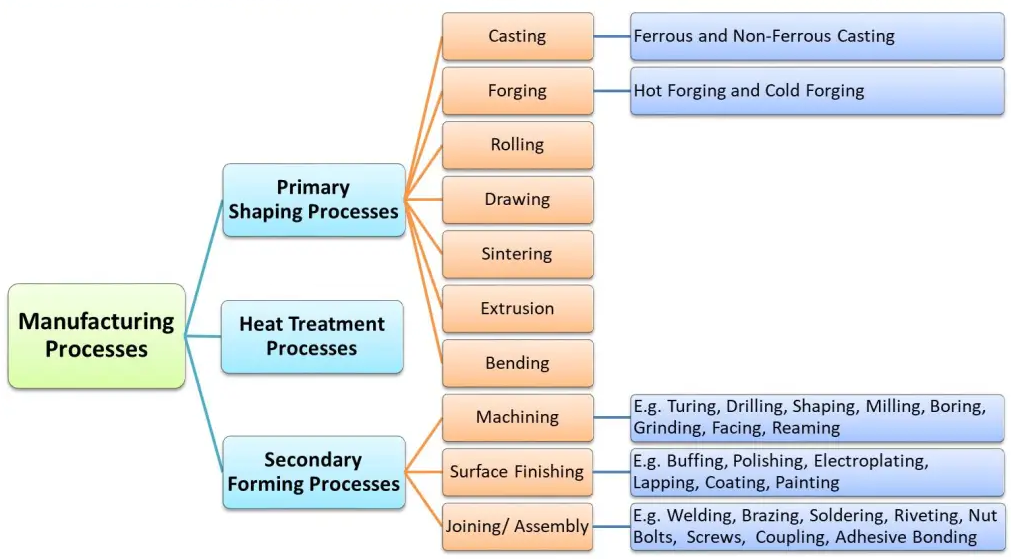
\includegraphics[height=6.5cm,width=1\textwidth,keepaspectratio]{fig2.png}
        \label{fig:fig2.png}
    \end{figure}
\end{frame}

\begin{frame}[t]{Videos for self education}
    \framesubtitle{}
    \vspace{-0.5cm}
    \small
    \begin{multicols}{2}
        \begin{enumerate}
            \item \href{https://youtu.be/Um_g8sQ_p3Y}{How Things Are Made | An Animated Introduction to Manufacturing Processes}
            \item \href{https://www.youtube.com/watch?v=SecY2IaMtfs}{UNBELIEVABLY FAST! High-Speed CNC Machining}
            \item \href{https://www.youtube.com/shorts/AN7u5P2_PWk}{CNC turning thread with high speed}
            \item \href{https://www.youtube.com/shorts/ODOPA6p55MI}{High-speed CNC milling!}
            \item \href{https://www.youtube.com/watch?v=AWoBKAUw8hQ}{CNC Water Jet Cutting Machine}
            \item \href{https://www.youtube.com/watch?v=s94KgsbGmzc}{SLA 3D printers}
            \item \href{https://www.youtube.com/watch?v=YdmY48lizR8}{SLS 3D Printer}
            \item \href{https://www.youtube.com/watch?v=h6fQVOiwuIY}{Keyway Cutting on Shaper Machine (Долбяк)}
            \item \href{https://www.youtube.com/shorts/jdDPIU-2fQo}{RPM 3500 with Steel. Fast but Waste Tools}
            \item \href{https://www.youtube.com/watch?v=i-PgeWbDgq4}{5D Milling machine}
            \item \href{https://www.youtube.com/shorts/gGnoeD1k9ck}{Z-MaT F855 High speed Vertical Machining Center}
            \item \href{https://www.youtube.com/shorts/Hk269KvcYs4}{Metal bird. CNC machining. 5-axis machining.}
            \item \href{https://www.youtube.com/watch?v=L1D5DLWWMp8}{Electrical Discharge Machining}
            \item \href{https://www.youtube.com/watch?v=5CeCxkFVCdM}{EDM Machine at home}
            \item \href{https://www.youtube.com/shorts/SNCGf3W5otE}{Result of EDM Machining}
        \end{enumerate}
    \end{multicols}
    

    % 
\end{frame}

    \begin{frame}[t]{Invited Lecturer Seif (ENG)}
        \framesubtitle{Video, Part 1}
        \vspace{-0.6cm}
        \begin{figure}[H]
            \href{https://disk.yandex.ru/i/ZSzrG8Uh0G7yvg}{
                \centering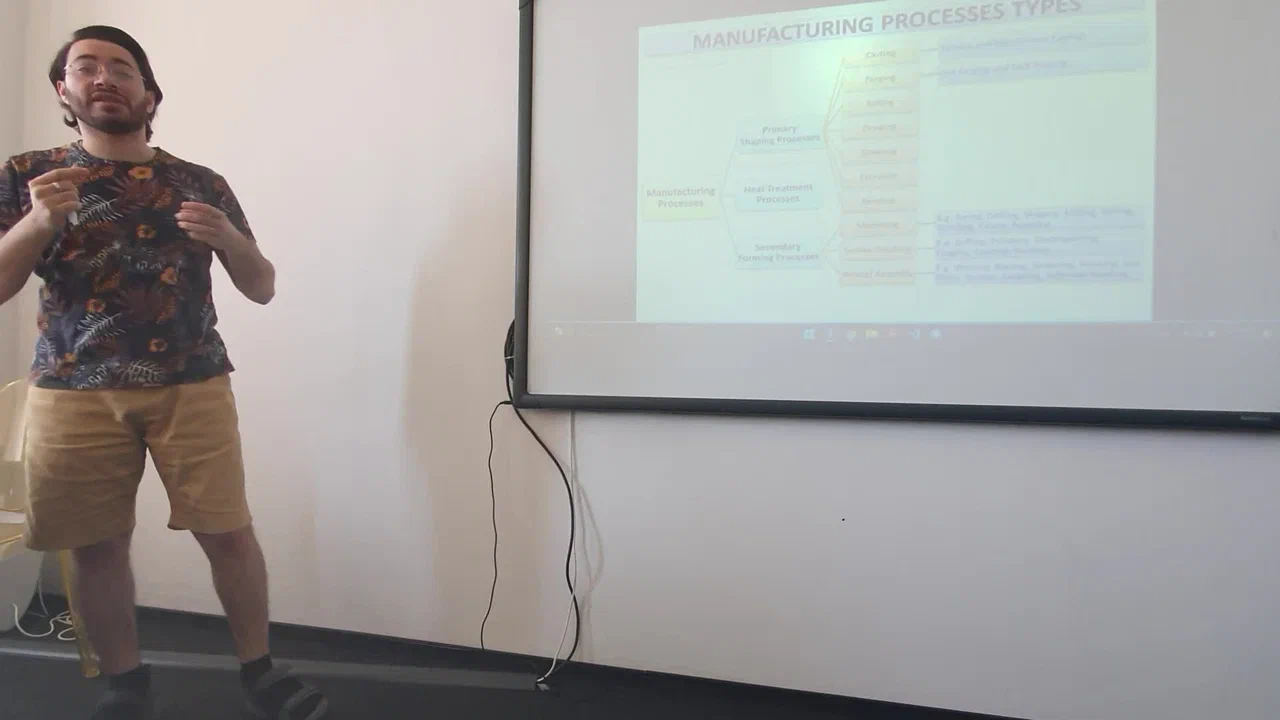
\includegraphics[height=6cm,width=1\textwidth,keepaspectratio]{seif_manufactoring_1_video.png}}
            \label{fig:seif_manufactoring_1_video.png}
        \end{figure}
    \end{frame}
    
    \begin{frame}[t]{Invited Lecturer Seif (ENG)}
        \framesubtitle{Video, Part 2}
        \vspace{-0.6cm}
        \begin{figure}[H]
            \href{https://disk.yandex.ru/i/ocx0EwLLyuIUHg}{
                \centering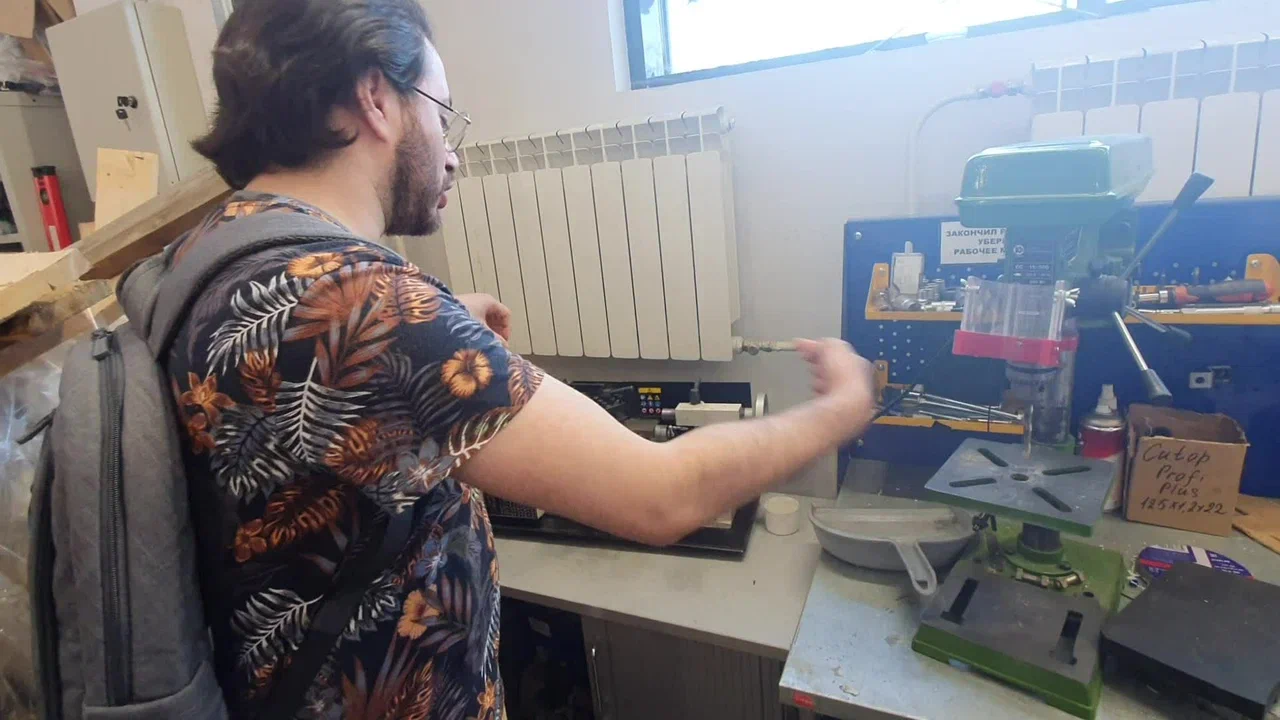
\includegraphics[height=6cm,width=1\textwidth,keepaspectratio]{seif_manufactoring_2_video.png}}
            \label{fig:seif_manufactoring_2_video.png}
        \end{figure}
    \end{frame}


\fbckg{fibeamer/figs/last_page.png}
\frame[plain]{}

\end{document}